\section{Summary}

We have investigated the possibility of determining the neutral pion
polarizabilities $\alpha_{\pi^0}-\beta_{\pi^0}$ by making a
measurement of the cross section of the Primakoff reaction $\gamma
\rm{Pb}\rightarrow \pi^0 \pi^0 \rm{Pb}$. We propose to make this
measurement using data taken simultaneously with the CPP\cite{CPPexp}
experiment in Hall D. The existing GlueX detector has sufficient
resolution and high acceptance for this process. We expect to collect approximately 3000 signal events during the
approved 20 PAC days. The anticipated statistical uncertainties on
the signal represent a significant improvement over existing data as shown in Fig.\,\ref{fig:sigma_2pi0_figs_4}.

\begin{figure}[tpb]
\centering
\includegraphics[page=4,width=4.75in]{figures/sigma_2pi0_figs.pdf}
\caption{Estimated statistical uncertainties on determining $\sigma(\gamma\gamma\rightarrow\pi^0\pi^0$) in the absence of background during 20 PAC days running simultaneously with the approved CPP experiment. The data points from the single previous measurement
are shown for comparison.
\label{fig:sigma_2pi0_figs_4}}
\end{figure}

The current estimate by Dai and Pennington \cite{Dai:2016ytz} indicates
that a 1.3\% determination of
$\sigma(\gamma\gamma\rightarrow\pi^0\pi^0)$ will determine the
combination $\alpha_{\pi^0}-\beta_{\pi^0}$ to a precision of 10\%,
but this estimate may be improved in the future with more kinematic-specific analysis. The theoretical work to model and to understand the backgrounds, such as
hadronic $t$-exchange involving $\rho^0$ and $\omega$, is ongoing.
